\subsection{Optimisation of a single constraint}
The first challenge in producing a library of virtual constraints is to produce a method by which a single constraint may be optimised -- the optimality of a planned trajectory cannot exceed the optimality of the primitives which compose it. The definition of optimality in the case of a bipedal robot is not clear; {\color{red}<insert literature references to competing definitions>}. \\

The definition of optimality chosen for the purposes of producing the virtual constraint library is as follows: \\

\emph{The optimal constraint for a given start and end configuration and kinetic energy gain or loss is the one which requires the minimum RMS torque value to maintain.} \\

Using this definition, we may further motivate the need for optimisation of the virtual constraints by way of example. Consider Figure \ref{fig:manualgen}; the constraint has been chosen based upon reasoning that it appears to produce a net-gain kinetic energy in a fairly smooth motion. However, the torque required to maintain this motion is clearly wasteful and nonmonotonic. {\color{red} Maybe try to give some good justification here.}

\begin{figure}
	\centering
	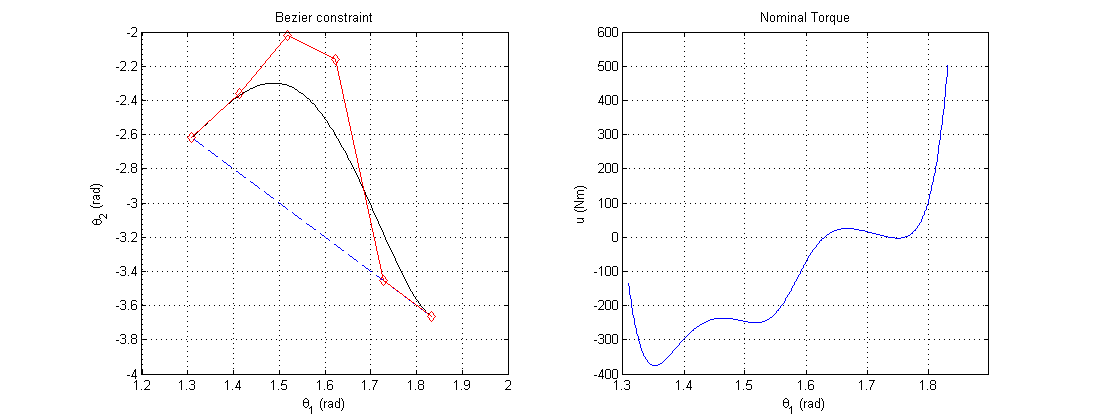
\includegraphics[width=0.9\linewidth]{4VirtConstLib/manualgen.png}
	\caption{Torque curve for manually generated constraint}
	\label{fig:manualgen}
\end{figure}

Unfortunately, the torque required to maintain a constraint varies with initial velocity. Since the virtual constraint library is prepared off-line, the initial velocity is unknown. The constraint is therefore optimised over a nominal trajectory. That is, each virtual constraint is only perfectly optimised for a particular initial velocity. {\color{red} Justify this, and go into depth about the choice of initial velocity? There's no reason that this should be the same per constraint. The nominal trajectory is probably different for each constraint.}

{\color{red} Also need to include constraints - friction cone and invariance. Also, perhaps discuss using time basis/using theta basis; theta basis may be skewed since it is not linear in time, so integral of torque as a function of theta gives a different result to integral of torque as a function of time. We can derive time-based torque at the cost of additional computation}

\subsection{Optimisation of library coverage}
Optimising a particular constraint for minimum torque is valuable for the achievement of efficient periodic walking on flat ground, however coverage over the configuration space of the robot is required for walking over uneven terrain and deliberate alterations in kinetic energy. Therefore, we require a method by which coverage of the configuration space with optimised constraints which achieve additions and subtractions of kinetic energy.